\documentclass[12pt]{article}
\title{EE445M Lab 2}
\author{Hershal Bhave (hb6279) and Eric Crosson (esc625)}
\date{Due Sometime Soon}

\usepackage[in]{fullpage}
\usepackage{listings}
\usepackage{cleveref}
\usepackage[nosolutionfiles]{answers}
\usepackage{graphicx}
\usepackage{xcolor}
\usepackage{color}
\usepackage{enumerate}

\newenvironment{Ex}{\textbf{Problem}\vspace{.75em}\\}{}
\Newassociation{solution}{Soln}{Answers}
\pagebreak[3]
\newcommand{\Opentesthook}[2]{\Writetofile{#1}{\protect\section{#1: #2}}}
\renewcommand{\Solnlabel}[1]{\textbf{Solution}\quad}
\newcommand{\todo}{{\LARGE \emph{\color{red}TODO}}}

\newcommand{\dd}[1]{\:\mathrm{d}{#1}}
\newcommand{\ddt}[1]{\frac{\dd{}}{\dd{#1}}}
\newcommand{\dddt}[1]{\frac{\dd{}^2}{\dd{#1}^2}}

\definecolor{mygreen}{rgb}{0,0.6,0}
% \definecolor{mygreen}{rgb}{0.13,0.55,0.13}
\definecolor{mygray}{rgb}{0.5,0.5,0.5}
\definecolor{mymauve}{rgb}{0.58,0,0.82}

\lstset{
  backgroundcolor=\color{white},
  basicstyle=\scriptsize\ttfamily,
  breakatwhitespace=false,
  breaklines=true,
  captionpos=b,
  commentstyle=\color{mygreen},
  deletekeywords={...},
  escapeinside={\%*}{*)},
  extendedchars=true,
  frame=single,
  keywordstyle=\color{blue},
  % language=Octave,
  % numbers=left,
  % numbersep=5pt,
  % numberstyle=\tiny\color{mygray},
  rulecolor=\color{black},
  showspaces=false,
  showstringspaces=false,
  showtabs=false,
  % stepnumber=2,
  stringstyle=\color{mymauve},
  tabsize=2,
  title=\lstname,
  columns=fullflexible,
}

\begin{document}
\maketitle

\section{Objectives}
{\huge \color{red} TODO}

\section{Hardware Design}
No hardware design required for this lab.

\section{Software Design}
{\huge \color{red} TODO}

\section{Measurement Data}
\begin{enumerate}
\item Reference \cref{fig:context-switch,fig:uart-consumer}.

  \graphicspath{../images}
  \begin{figure}
    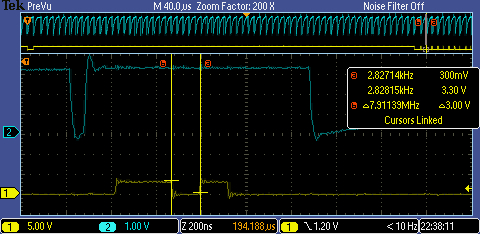
\includegraphics{TEK00001}
    \caption{A context switch}
    \label{fig:context-switch}
  \end{figure}
  \begin{figure}
    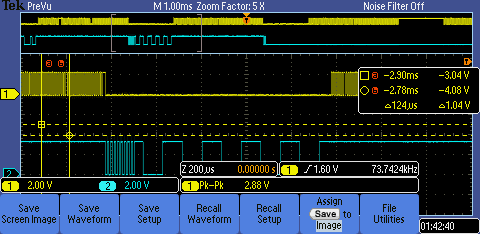
\includegraphics{TEK00000}
    \caption{Retrieving data from the UART FIFO. The blue line
      represents the UART consumer thread consuming UART data from the
      FIFO, the yellow line represents all other threads. You can
      clearly see the UART consumer thread retrieving data in the FIFO
      in quick succession, and then waiting for real-time data to
      arrive}
    \label{fig:uart-consumer}
  \end{figure}

\item Measurement of the Thread-Switch Time:

  The thread-switch takes less than 7$\mu$s to complete.
\item Reference \cref{fig:context-switch,fig:uart-consumer}.
\item This is what the circular linked list looks like before, after,
  and during a thread switch. The TCB pointed to by
  \verb|os_running_threads| circulates through the TCB data
  structures, as shown in \verb|$12| by the \verb|next| TCB variable.

\begin{verbatim}
  (gdb) p *os_running_threads
$9 = {
  sp = 0x200008a0 <OS_PROGRAM_STACKS+732>,
  next = 0x2000058c <OS_THREADS+56>,
  prev = 0x200005a8 <OS_THREADS+84>,
  id = 1,
  entry_point = 0x6e1 <uart_consumer>,
  status = THREAD_RUNNING,
  sleep_timer = 0
}
(gdb) p *os_running_threads->next
$10 = {
  sp = 0x20000a30 <OS_PROGRAM_STACKS+1132>,
  next = 0x200005a8 <OS_THREADS+84>,
  prev = 0x20000570 <OS_THREADS+28>,
  id = 2,
  entry_point = 0x651 <Thread2>,
  status = THREAD_RUNNING,
  sleep_timer = 0
}
(gdb) p *os_running_threads->next->next
$11 = {
  sp = 0x20000bc0 <OS_PROGRAM_STACKS+1532>,
  next = 0x20000570 <OS_THREADS+28>,
  prev = 0x2000058c <OS_THREADS+56>,
  id = 3,
  entry_point = 0x619 <Thread1>,
  status = THREAD_RUNNING,
  sleep_timer = 0
}
(gdb) p *os_running_threads->next->next->next
$12 = {
  sp = 0x200008a0 <OS_PROGRAM_STACKS+732>,
  next = 0x2000058c <OS_THREADS+56>,
  prev = 0x200005a8 <OS_THREADS+84>,
  id = 1,
  entry_point = 0x6e1 <uart_consumer>,
  status = THREAD_RUNNING,
  sleep_timer = 0
}
(gdb)
\end{verbatim}

\item  Reference \cref{tab:fifo-perf}.
  \begin{table}[h]
    \centering
    \begin{tabular}[H]{c|c|c|c|c}
           & 32 & 64 & 128 & 256 \\ \hline
      500  & 8  & 4  & 2   & 0   \\ \hline
      1000 & 6  & 3  & 0   & 0   \\ \hline
    \end{tabular}
    \caption{Context Switch Frequency (Hz) vs. UART Buffer FIFO Overwrites}
    \label{tab:fifo-perf}
  \end{table}
\item Reference \cref{tab:debugging-instruments-perf}.
  \begin{table}[h]
    \centering
    \begin{tabular}[H]{c|c}
      With Debugging Instruments & 1224 \\ \hline
      Without Debugging Instruments & 12300 \\
    \end{tabular}
    \caption{Context Switch Frequency (Hz) vs. UART Buffer FIFO Overwrites}
    \label{tab:debugging-instruments-perf}
  \end{table}
  The value of \verb|PIDWork| without debugging instruments is
    12300, the value with debugging instruments is 1224.
\end{enumerate}

\section{Analysis and Discussion}
\begin{enumerate}
\item {\huge \color{red} TODO}
\end{enumerate}

\end{document}
